

	\section{Материалы}
	
	
	
	\section{РСА}
	
	\subsection{Почему этот метод}
	когерентность и здоровая статистика
	
	
	\subsection{Схема эксперимента}
	
	
	
	\subsection{Обработка резлультатов}
	
	\paragraph{интегрирование распознавание пиков}
	че получили:
		\begin{figure}
    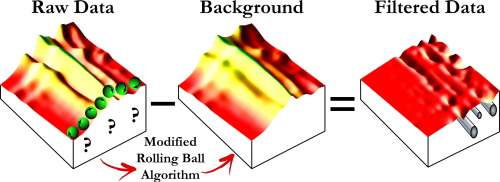
\includegraphics[width=\textwidth]{fig/rolling-ball.jpg}
    \caption{Принцип работы алгоритма}
    \label{fig:rolling-ball}
\end{figure}
	
	\paragraph{Rolling-ball}
	погрешности, чем хорошо, почему он, какие еще бывают
	
	А код - в приложении!
	
	\begin{figure}
    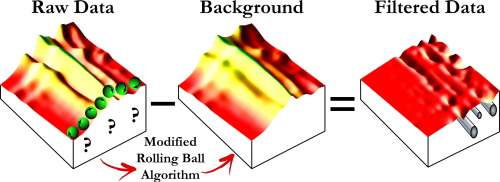
\includegraphics[width=\textwidth]{fig/rolling-ball.jpg}
    \caption{Принцип работы алгоритма}
    \label{fig:rolling-ball}
\end{figure}

    \paragraph{фиттинг}

\begin{figure}
    \centering
    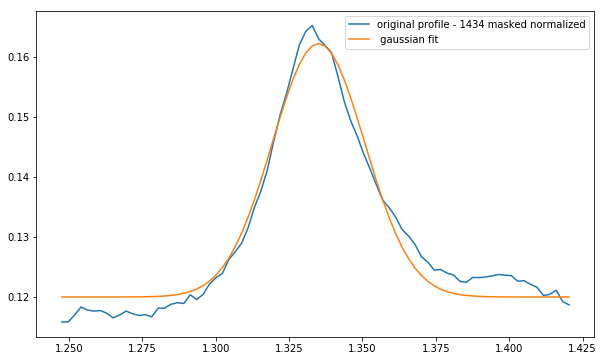
\includegraphics[width=\linewidth]{fig/gauss-fit.png}
    \caption{Аппроксимация формы пика по разным моделям}
    \label{fig:my_label}
\end{figure}
	
	\paragraph{Карты кристалличности}
	
	\begin{figure}[ht]\center
\begin{tabular}{cc}
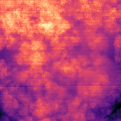
\includegraphics[width=0.5\linewidth]{fig/map-1.png}
&
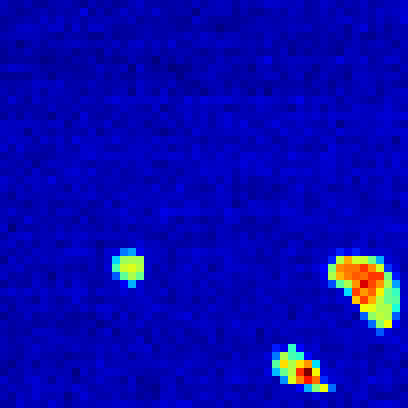
\includegraphics[width=0.5\linewidth]{fig/map-2.png}
\end{tabular}
\caption{Карты кристалличности}
\end{figure}
	
	

	
	
	
	Свойства и результаты прочих исследований:
	[Vaganov corrected]